%Talk given at Matrix, June 12, 2018
\documentclass[10pt,compress,xcolor={usenames,dvipsnames},aspectratio=169]{beamer} %slides and 
%notes
\usepackage{amsmath,datetime,
	mathtools,
	bbm,
%	mathabx,
	array,
	booktabs,
	mcode,
	alltt,
	xspace,
	calc,
	colortbl,
	graphicx}
\usepackage[usenames]{xcolor}
\usepackage[style=nature]{biblatex}
\addbibresource{FJHown23.bib}
\addbibresource{FJH23.bib}
\usepackage{newpxtext}
\usepackage[euler-digits,euler-hat-accent]{eulervm}
\usepackage{media9}
%\usepackage{cleveref}
\usetheme{FJHSlimNoFoot169}


\setlength{\parskip}{2ex}
\setlength{\arraycolsep}{0.5ex}


\title[]{Automatic Algorithms for Multidimensional Integration}
\author[]{Fred J. Hickernell}
\institute{Department of Applied Mathematics \\
	Center for Interdisciplinary Scientific Computation \\  Illinois Institute of Technology \\
	\href{mailto:hickernell@iit.edu}{\url{hickernell@iit.edu}} \quad
	\href{http://mypages.iit.edu/~hickernell}{\url{mypages.iit.edu/~hickernell}}}
\thanksnote{Thanks to the GAIL team, esp.\ Lan Jiang, Llu\'is Antoni Jim\'enez Rugama, and Jagadees Rathinavel \\ NSF-DMS-1522687 and NSF-DMS-1638521 (SAMSI)
}
\event{Matrix Workshop on the Frontiers of High Dimensional Computation}
\date[]{June 11, 2018}

\iffalse

Abstract:  We review recent algorithms designed to automatically terminate when the error tolerance has been reached.  There are algorithms based on IID sampling and low discrepancy sampling.  The underlying function may be assumed to be deterministic or an instance of a Gaussian process.  We describe the theory behind these algorithms and illustrate their performance via examples.

\fi

\input FJHDef.tex
\renewcommand{\mSigma}{\Sigma}
\newcommand{\tol}{\text{tol}}
\newcommand{\Phnu}{\Prob_{\hnu}}
\DeclareMathOperator{\hugetext}{huge}
\DeclareMathOperator{\oerr}{\overline{err}}
\DeclareMathOperator{\cubMC}{cubMC}
\DeclareMathOperator{\qse}{qse}
\DeclareMathOperator{\integ}{int}
\DeclareMathOperator{\trap}{trap}
\DeclareMathOperator{\size}{size}
\DeclareMathOperator{\app}{id}
\DeclareMathOperator{\err}{err}
\DeclareMathOperator{\MSE}{MSE}
\DeclareMathOperator{\RMSE}{RMSE}
\DeclareMathOperator{\PProb}{\mathbb{P}}
\DeclareMathOperator{\walsh}{walsh}
\newcommand{\happ}{\widehat{\app}}
\newcommand{\hinteg}{\widehat{\integ}}
\newcommand{\cube}{[0,1)^d}
\newcommand{\desall}{\{\vz_i\}}
\newcommand{\desn}{\{\vz_i\}_{i=0}^{n-1}}
\def\newblock{\hskip .11em plus .33em minus .07em}
\newcommand{\wcS}{\widecheck{S}}
\newcommand{\wcomega}{\widecheck{\omega}}
\newcommand{\HickernellFJ}{H.} %To give my name to the bibliography
\newcommand{\abstol}{\varepsilon_{\textup{a}}}
\newcommand{\reltol}{\varepsilon_{\textup{r}}}
\DeclareMathOperator{\MLE}{MLE}
\DeclareMathOperator{\algn}{ALN}
\DeclareMathOperator{\disc}{disc}
\DeclareMathOperator{\Var}{Var}
\DeclareMathOperator{\RMS}{RMS}
\DeclareMathOperator{\GP}{\cg\cp}
\newcommand{\Dt}{\text{D}}
%\newcommand{\Rn}{\text{R}}
\newcommand{\Ba}{\text{B}}
\newcommand{\tmC}{\widetilde{\mC}}
\newcommand{\tvC}{\widetilde{\vC}}
\newcommand{\vC}{\boldsymbol{C}}
\newcommand{\hvtheta}{\hat{\vtheta}}
\newcommand{\hc}{\widehat{c}}
\newcommand{\hvc}{\widehat{\vc}}
\newcommand{\hs}{\hat{s}}
\newcommand{\hvz}{\widehat{\vz}}
\renewcommand{\tmu}{\widetilde{\mu}}
\DeclareMathOperator{\sol}{sol}
\DeclareMathOperator{\hsol}{\widehat{\sol}}
\DeclareMathOperator{\appx}{app}


\definecolor{MATLABBlue}{rgb}{0, 0.447, 0.741}
\definecolor{MATLABOrange}{rgb}{0.85,  0.325, 0.098}
\definecolor{MATLABPurple}{rgb}{0.494,  0.184, 0.556}
\definecolor{MATLABGreen}{rgb}{0.466,  0.674, 0.188}

\newcommand{\GaussPict}{\href{http://www.mathworks.com/matlabcentral/answers/uploaded_files/26298/Plotting\%20a\%203d\%20gaussian\%20function\%20using\%20surf\%20-\%202015\%2002\%2027.png}
	{\includegraphics[height
		= 1.8cm]{Programs/Plotting_gaussian.png}}}

\newcommand{\financePict}{\href{http://i2.cdn.turner.com/money/dam/assets/130611131918-chicago-board-options-exchange-1024x576.jpg}{\includegraphics[width
		= 
		3cm]{Programs/130611131918-chicago-board-options-exchange-1024x576.jpg}}}

\begin{document}
\everymath{\displaystyle}

\frame{\titlepage}



\section{Introduction}

\begin{frame}
\frametitle{When Do We Stop?}
\vspace{-2ex}

Compute an \alert{integral}
\begin{equation*}
\mu(f) =  \int_{\reals^d} f(\vx) \, \varrho(\vx) \, \dif \vx \qquad  \text{Bayesian inference, financial risk, statistical physics, \ldots} 
\end{equation*} 
\alert{Desired solution:}  An adaptive algorithm, $\hmu(\cdot, \cdot)$ of the form
\[
\hmu(f, \varepsilon)  =  w_{0,n} +  \sum_{i=1}^n w_{i,n} f(\vx_i), \qquad \text{e.g., } w_{0,n} = 0,  \ w_{1,n} = \cdots = w_{n,n} = \frac 1n 
\]
where \alert{$n$}, $\{\vx_i\}_{i=1}^{\infty}$, $w_{0,n}$, and $\vw = (w_{i,n})_{i=1}^n$  are chosen to \alert{guarantee}
\[
\bigabs{\mu(f) - \hmu(f,\varepsilon)} \le \varepsilon \text{ with high probability}\qquad \forall \varepsilon > 0,  \text{ \alert{reasonable} } f
\]

\end{frame}


\begin{frame}
\frametitle{When Do We Stop?}
\vspace{-8ex}
 
\begin{gather*}
\mu(f) =  \int_{\reals^d} f(\vx) \, \varrho(\vx) \, \dif \vx, \qquad \hmu(f, \varepsilon)  =  w_{0,n} +  \sum_{i=1}^n w_{i,n} f(\vx_i), \\
\text{Want} \quad \bigabs{\mu(f) - \hmu(f,\varepsilon)} \le \varepsilon \text{ with high probability}\qquad \forall \varepsilon > 0,  \text{ \alert{reasonable} } f
\end{gather*}
\begin{tabular}{>{\raggedright}m{0.55\textwidth}>{\raggedright}m{0.4\textwidth}}
Possible solutions & Drawbacks \tabularnewline
\toprule
\alert{IID} sampling: $
n = \left(\frac{2.58 \hsigma}{\varepsilon}\right)^2
$
& 
Does CLT hold yet?  How to determine $\hsigma$?
\tabularnewline
\midrule
\alert{Low discrepancy} sampling:  choose $n$ to make $\disc(\{\vx_i\}_{i=1}^n) \Var(f) \le \varepsilon$
&
Don't know $\Var(f)$; computing $\disc(\{\vx_i\}_{i=1}^n)$ may be expensive
\tabularnewline
\midrule
\alert{Randomized low discrepancy} sampling: look at spread of sample means from random replications of low discrepancy points
&
How many replications?  What measure of spread?
\tabularnewline
\bottomrule
\uncover<2>{
\begin{itemize}
	
	\item Identify a data-driven measure of error
	
	\item Identify a \alert{cone} of nice integrands for which that data-driven error can be proven to hold
	
\end{itemize}}
&
\uncover<2>{ \vspace{-2ex} Is integrand really in the cone?

Well, sometimes there are necessary conditions that can be checked}
\end{tabular}

\end{frame}

\section{Algorithms So Far}

\begin{frame}
\frametitle{Automatic IID Sampling\footfullcite{HicEtal14a}}
\vspace{-4ex}
Replace the Central Limit Theorem by Berry-Esseen inequalities:
\begin{equation*}
\mu :=  \int_{\cx} f(\vx) \, \varrho(\vx) \dif\vx =: \Ex[f(\vX)], \qquad \cc = \{f \in L^4(\cx,\varrho) : \kurt(f(\vX)) \le \kappa_{\text{up}} \}
\end{equation*}
For $n_\sigma$ determined by $\kappa_{\text{up}}$, and $\vx_1, \vx_2, \ldots $ IID let 
\begin{gather*}
\sigma_{\text{up}}^2 = \frac{(1.2)^2}{n_\sigma-1} \sum_{i=1}^{n_\sigma}f(\vx_i), \qquad \hmu(f,\varepsilon) = \frac 1{n_\mu} \sum_{i=n_\sigma+1}^{n_\sigma + n_{\mu}} f(\vx_i), \quad\text{where}\\
n_\mu = \min \left\{n \in \naturals: 
\Phi\left(-\sqrt{n}\varepsilon/\sigma_{\text{up}} 
\right)+\frac{1}{\sqrt{n}} \min\left(0.3328(\kappa_{\text{up}}^{3/4}+0.429), \frac{18.1139 
	\kappa_{\text{up}}^{3/4}}{1+\abs{\sqrt{n}\delta/\sigma_{\text{up}}}^{3}} 
\right) \le 0.25\% \right\}
\end{gather*}
Then $\Prob\{\abs{\mu(f) - \hmu(f,\varepsilon)} \le \varepsilon\} \ge 99\%$.
\end{frame}

\begin{frame}[fragile]
\frametitle{Automatic Quasi-Monte Carlo Sampling\footfullcite{HicJim16a,JimHic16a,HicEtal17a}}
%\footfullcite{}
\vspace{-7ex}
\begin{gather*}
\mu = \int_{[0,1]^d} f(\vx) \, \dif \vx = \hf(\vzero), \qquad f(\vx) = \sum_{\vk} \hf(\vk) \phi_\vk(\vx), \quad \hf(\vk) = \int_{[0,1]^d} f(\vx) \overline{\phi}_{\vk}(\vx)\, \dif \vx\\  \phi_\vk \text{ are complex exponentials (for lattices) or Walsh functions (for nets)} \\
\cc = \text{ integrands whose true Fourier coefficients do not decay erratically}
\end{gather*}
The error bound is derived in terms of 
	\begin{gather*}
	\text{discrete transform, } \tf_n(\vk) = \frac 1n \sum_{i=1}^n f(\vx_i) \overline{\phi}_\vk(\vx_i) \ \forall \vk, \text{ can be computed in } \Order(n \log(n)) \text{ operations} \\
	\fC(n) \sum_{\text{moderate} \vk} \abs{\tf_n(\vk)} \le \varepsilon \implies \abs{\mu(f) - \hmu(f,\varepsilon)} \le \varepsilon
	\end{gather*}
\end{frame}

\begin{frame}
\frametitle{Integrands Inside and Outside the Cone}
%\vspace{-5ex}

\centerline{
\includegraphics[width = 0.32\textwidth] 
{Programs/FunctionWalshFourierCoeffDecay.eps} \qquad 
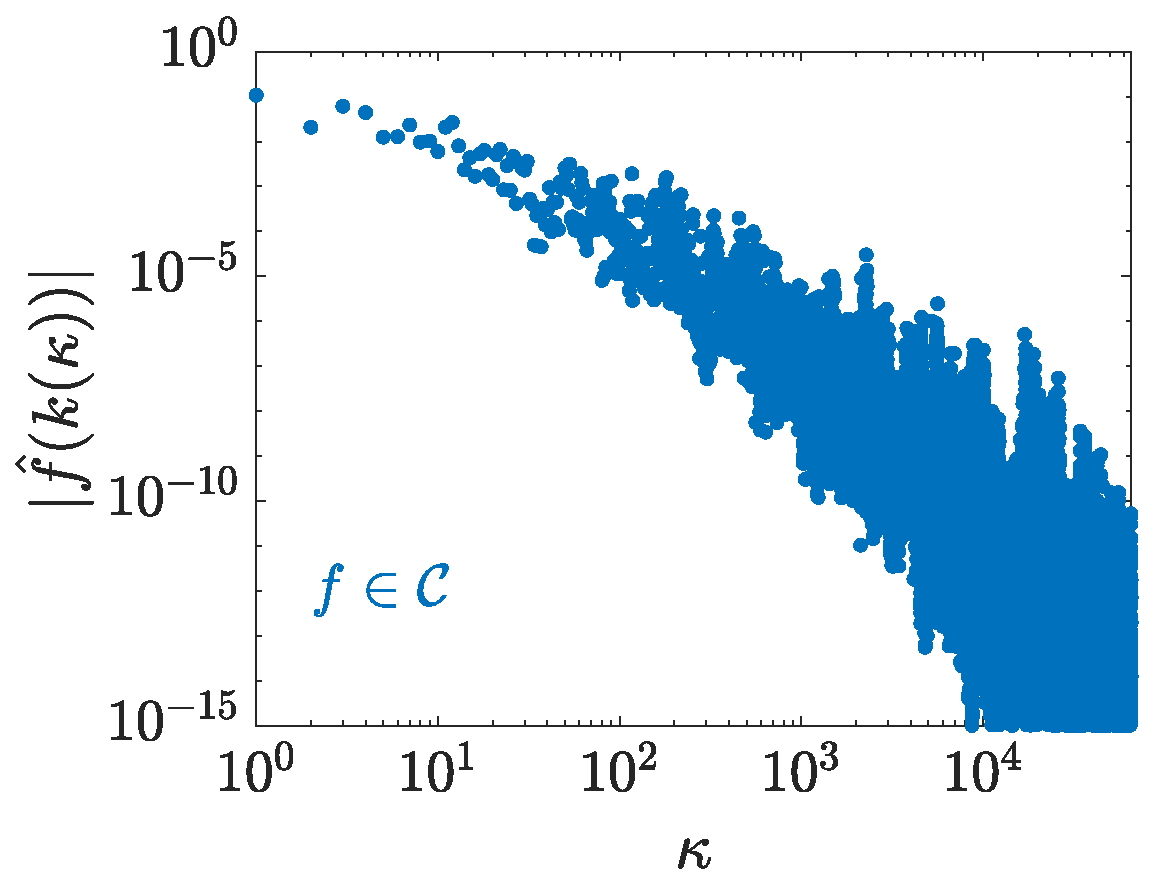
\includegraphics[width = 0.32\textwidth] 
{Programs/WalshFourierCoeffDecay128.eps}}

\centerline{
\includegraphics[width = 0.32\textwidth] 
{Programs/FilteredFunctionWalshFourierCoeffDecay.eps} \qquad
\includegraphics[width = 0.32\textwidth] 
{Programs/WalshFourierCoeffDecayFilter.eps}}
{\tiny }
\end{frame}

\begin{frame}
\frametitle{Automatic QMC Sampling Assuming a Random $f$}
\vspace{-3ex}
\alert{Assume } $f \sim \GP(m,s^2C_{\vtheta})$, a sample from a Gaussian process.  Defining

\vspace{-5ex}
\begin{equation*}
c = \int_{[0,1]^d} \int_{[0,1]^d} C_{\vtheta}(\vt,\vx) \, \dif \vt \dif \vx, \qquad 
\vc = \left(\int_{[0,1]^d}  C_{\vtheta}(\vt,\vx_i) \, \dif \vt  \right)_{i=1}^n , \qquad
\mC = \bigl(C_{\vtheta}(\vx_i,\vx_j)  \bigr)_{i,j=1}^n
\end{equation*}
and choosing the \alert{weights} as
\begin{equation*}
w_0 = m[ 1 - \vc^T \mC^{-1}\vone], \quad \vw = \mC^{-1} \vc, \qquad \hmu(f, \varepsilon)  = w_0 + \vw^T\vf,
\quad \vf = \bigl ( f(\vx_i) \bigr)_{i=1}^n.
\end{equation*}
yields an unbiased approximation:
\begin{equation*}
\mu(f) - \hmu(f,\varepsilon) \, \big \vert \, \vf = \vy \sim \cn\Bigl( 0, s^2(c - \vc^T \mC^{-1}\vc)\Bigr)
\end{equation*}
Choosing $n$  large enough to make 
\begin{equation*}
2.58s\sqrt{c - \vc^T \mC^{-1}\vc} \le \varepsilon,
\end{equation*}
 \alert{assures} us that 
\begin{equation*}
\Prob_{f} \left[\abs{ \mu(f) - \hmu(f,\varepsilon) } \le \varepsilon \right] \ge 99\%.
\end{equation*}
	\alert{Issues requiring attention:}  choosing parameters of the covariance kernel, expensive matrix operations
\end{frame}

\begin{frame}
\frametitle{To Make This Approach Practical\footfullcite{RatHic19a}}
\vspace{-4ex}
\begin{itemize}
	\item Use MLE to estimate parameters
	
	\item Choose covariance kernels that \alert{match the low discrepancy design}
	\begin{gather*}
	c = \int_{[0,1]^d} \int_{[0,1]^d} C_{\vtheta}(\vt,\vx) \, \dif \vt \dif \vx = 1, \qquad \vc = \left(\int_{[0,1]^d}  C_{\vtheta}(\vt,\vx_i) \, \dif \vt  \right)_{i=1}^n = \vone \\
	 \mC = \Bigl( C_{\vtheta}(\vx_i, \vx_j) \Bigr)_{i,j=1}^n = \frac 1n \mV \mLambda \mV^H, 
	\quad \mLambda = \diag(\vlambda), \quad \alert{\vV_1 = \vv_1 = \vone} \\
	\mV^T \vz \alert{\text{ is }\Order(n \log n)}, \qquad \vlambda = \mV^T \vC_1, \qquad \mC^{-1} \vone = \frac{\vone}{\lambda_1}
	\end{gather*} 	
	
\end{itemize}

\vspace{-3ex}

Dealing with the \alert{fast transformed} data, $\hvy = \mV^T \vy$, where $\vy = \bigl ( f(\vx_i) \bigr)_{i=1}^n$, it follows that 

\vspace{-5ex}

\begin{gather*}
\hmu(f,\varepsilon) =  \frac{\hy_1}{n} = \frac 1n \sum_{i=1}^n f(\vx_i), \qquad  
\Prob_{f} \left[\abs{ \mu(f) - \hmu(f,\varepsilon) } \le \varepsilon \right] \ge 99\%., \\
\text{provided } \qquad 
2.58\sqrt{\left(1 - \frac{n}{\lambda_1}\right)
	\frac 1{n^2} \sum_{i=\alert{2}}^n \frac{\lvert \widehat{y}_i \rvert^2}{\lambda_i} } \le \varepsilon
\end{gather*}


\end{frame}

\begin{frame}
\frametitle{Form of Matching Covariance Kernels}
\vspace{-4ex}
Typically the domain of $f$ is $[0,1)^d$, and 
\begin{equation*}
C(\vt,\vx)  = \begin{cases}
\tC(\vx - \vt \bmod 1) & \text{integration lattices} \\
\tC(\vx \oplus \vt) & \text{Sobol' sequences},  \oplus \text{ means digitwise addition modulo } 2
\end{cases}
\end{equation*}
E.g., for integration lattices
\[
C(\vx,\vt) = \prod_{k=1}^d [1 - \theta_1 (-1)^{\theta_2}B_{2\theta_2}(x_k-t_k \bmod 1)], \qquad \theta_1 > 0,  \theta_2 \in \naturals
\]
\centerline{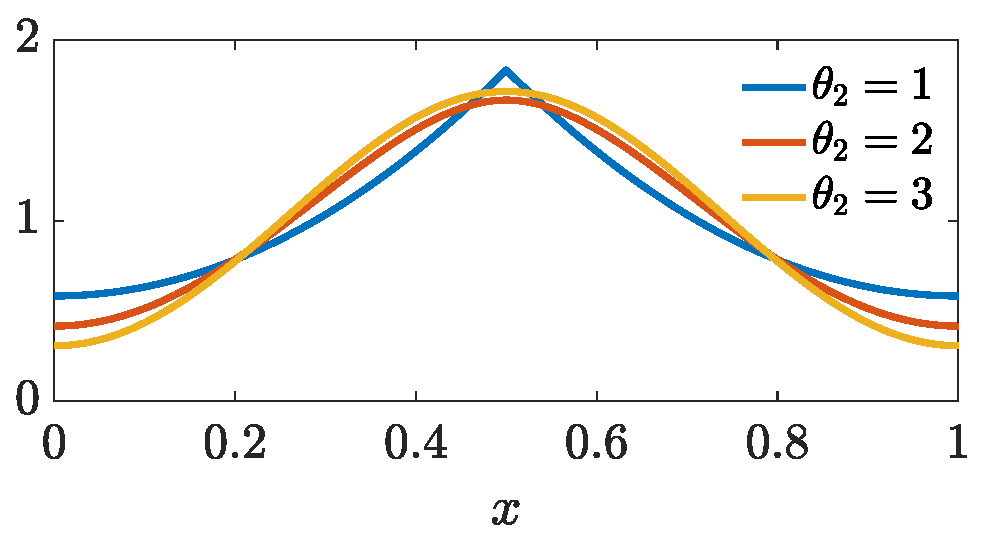
\includegraphics[width=0.5\textwidth]{Programs/BernoulliKernel.eps}}

\end{frame}


\section{Example}

\begin{frame}[label=GaussProb]
\frametitle{Gaussian Probability}
\vspace{-8ex}
\begin{tabular}{m{0.7\textwidth}m{3cm}}
	\begin{equation*}
	\mu = \int_{[\va,\vb]} \frac{\exp\bigl(- \frac 12 \vt^T \mSigma^{-1} \vt 
		\bigr)}{\sqrt{(2 
			\pi)^d \det(\mSigma)}} \, \dif \vt \
	= \ \int_{[0,1]^{d-1}} 
	f(\vx) \, 
	\dif \vx
	\end{equation*}
	& 
	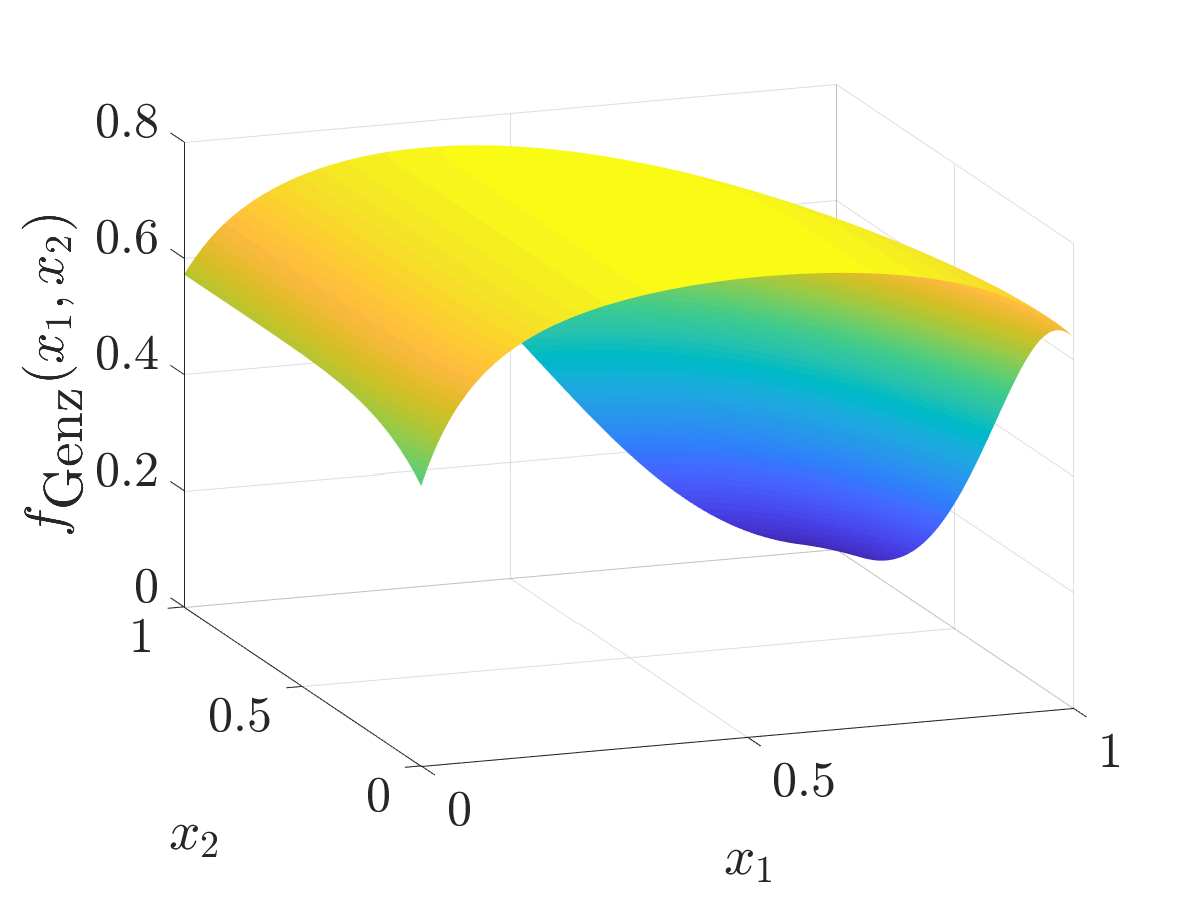
\includegraphics[height = 2.3cm]{Programs/GenzFun.eps}
\end{tabular}

\vspace{-4ex}
For some typical choice of 
$\va$, $\vb$, $\mSigma$, $d=3$;  $\mu \approx 0.6763$

\vspace{-4ex}

\begin{equation*}
\begin{array}{cccccc}
\text{\alert{Rel.}\ Error} & & \text{Median}&& \text{Worst 10\%} & \text{Worst 10\%} \\
\text{Tolerance} & \text{Method}  & \text{Error} & \text{Accuracy} 
& n & \text{Time (s)} \\
\toprule
\input{Programs/MVNFixedWidth.txt}
\end{array}
\end{equation*}

\vspace{-2ex}

These algorithms are implemented in GAIL\footfullcite{ChoEtal17b}
\end{frame}

\begin{frame}
\frametitle{ Option Pricing}
\vspace{-10ex}
\begin{tabular}{m{11cm}m{2.5cm}}
	\[
	\begin{aligned}
	\mu= \text{fair price} = 
	\int_{\reals^d}\me^{-r T}\max\left(\frac{1}{d}\sum_{j=1}^d S_{j}-K, 0\right) 
	\frac{\me^{-\vz^T\vz/2}}{(2\pi)^{d/2}}\,\dif \vz \approx \$13.12
	\end{aligned}
	\]
	& 
	\financePict
\end{tabular}
\vspace{-4ex}
\begin{gather*}
S_{j} =  S_0\me^{(r-\sigma^2/2)jT/d+\sigma x_j} = \text{stock price at time } 
jT/d, \\
\vx  = \mA \vz, \quad \mA \mA^T = \mSigma = \Bigl ( \min(i,j) T/d \Bigr) _{i,j = 1}^d,
\quad T = 1/4, \ d=13 \text{ here}
\end{gather*}
\begin{equation*}
\begin{array}{cccccccc}
\text{Abs.\ Error}& & & \text{Median}&& \text{Worst 10\%} & \text{Worst 10\%} \\
\text{Tolerance} & \multicolumn{2}{c}{\text{Method}}  & \text{Error} & \text{Accuracy} 
& n & \text{Time (s)} \\
\toprule
\input{Programs/AsianOutput.txt}
\end{array}
\end{equation*}
\vspace{-8ex}

\end{frame}

\section{What Comes Next}

\begin{frame}[fragile]
\frametitle{Future Work}

\vspace{-3ex}
\begin{itemize}
	\item Bayesian cubature with higher order nets and smoother kernels, control variates
	
	\item Stopping criteria for multilevel and multivariate decomposition methods
	
	\item Community QMC software that \alert{combines the efforts of several research groups}
	\begin{itemize}
		\item Skeleton with clearly defined properties for different kinds of objects
		
		\item Plug-and-play functionality
		
		\vspace{-2ex}
		
	
		\lstinputlisting{Programs/IntegrationExample.m}
		
		\begin{alltt}
			>> IntegrationExample
			sol =
			0.428567222603452
			sol =
			0.425203913946775
		\end{alltt}
		
	\end{itemize}
	
\end{itemize}
\end{frame}


\setlength{\FJHThankYouMessageOffset}{-10ex}

\finalthanksnote{Slides available on SpeakerDeck at
	\href{https://speakerdeck.com/fjhickernell/matrix-week-two-2018-june}
	{\nolinkurl{speakerdeck.com/fjhickernell/matrix-week-two-2018-june}}
}

\thankyouframe

\printbibliography



\end{document}







